
\documentclass{beamer}

\usetheme{focus} % see https://github.com/elauksap/focus-beamertheme
% Add option [numbering=none] to disable the footer progress bar
% Add option [numbering=fullbar] to show the footer progress bar as always full with a slide count

\usepackage{booktabs} % Required for better table rules

\title{Evolution of Ice Sheet Geometry using Stokes Dynamics}

%\subtitle{Subtitle}

\author{Ed Bueler}

\titlegraphic{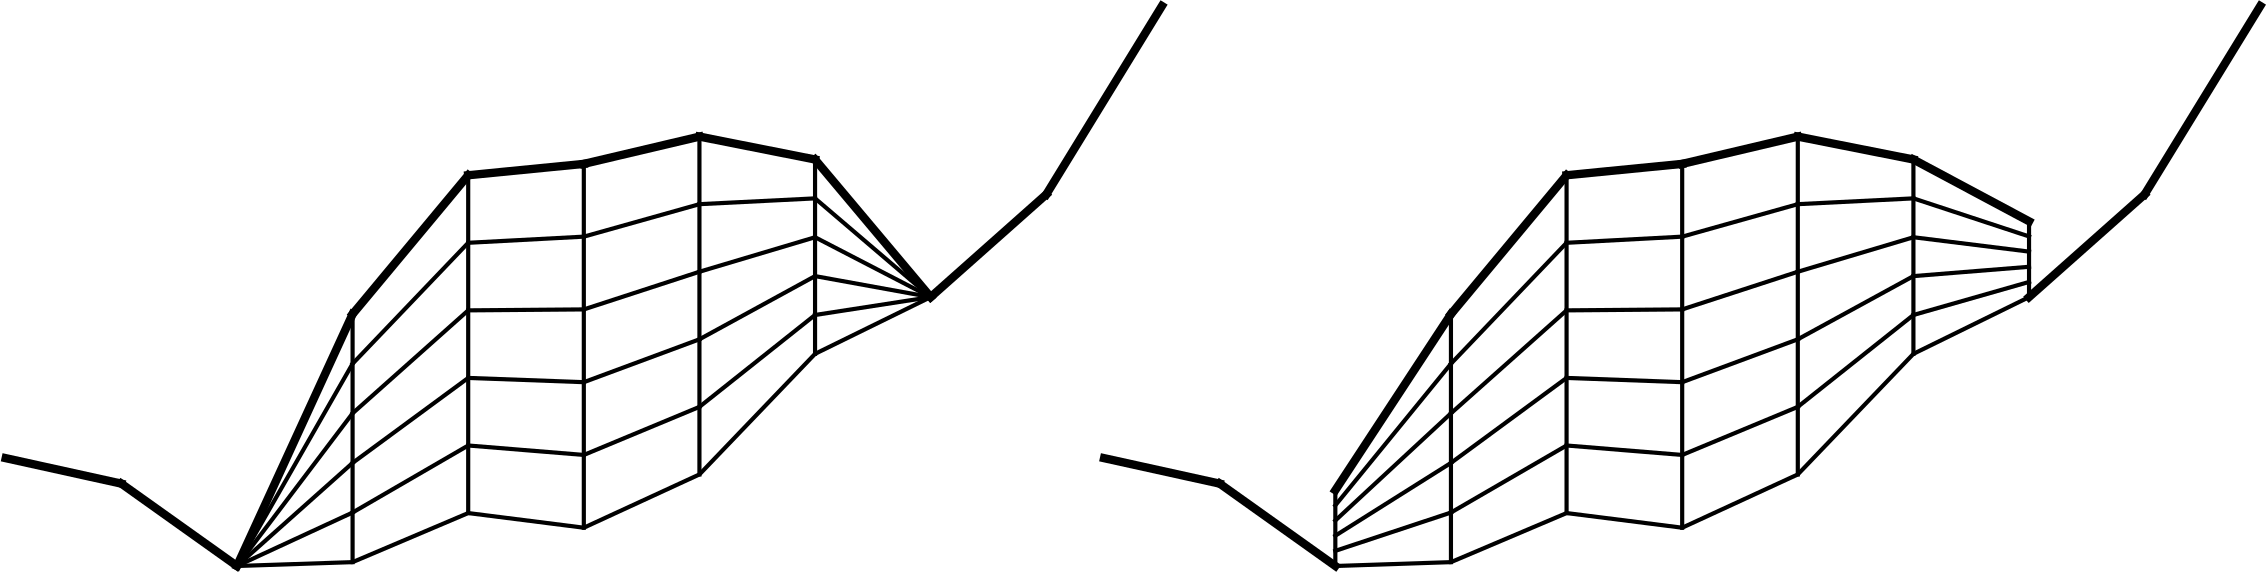
\includegraphics[width=0.55\textwidth]{figs/extruded.png} \\ 
\includegraphics[width=0.18\textwidth]{figs/uafbw.png}}

\institute{University of Alaska Fairbanks}

\date{\phantom{foo} \bigskip \bigskip \\ SIAM GS21 \\ with assistance from Lawrence Mitchell}


\begin{document}

\begin{frame}
	\maketitle
\end{frame}

\begin{frame}
	\tableofcontents
\end{frame}


\section{Section 1}

\begin{frame}{Typesetting and Math}
	The packages \texttt{inputenc} and \texttt{FiraSans}\footnote{\url{https://fonts.google.com/specimen/Fira+Sans}}\textsuperscript{,}\footnote{\url{http://mozilla.github.io/Fira/}} are used to properly set the main fonts.
	\vfill
	This theme provides styling commands to typeset \emph{emphasized}, \alert{alerted}, \textbf{bold}, \textcolor{example}{example text}, \dots
	\vfill
	\texttt{FiraSans} also provides support for mathematical symbols \cite{Bueler2021conservation}:
	\begin{equation*}
		e^{i\pi} + 1 = 0.
	\end{equation*}
\end{frame}


\section{Section 2}


\begin{frame}{Blocks}
	These blocks are part of 1 slide, to be displayed consecutively.
	\begin{block}{Block}
		Text.
	\end{block}
	\pause % Automatically creates a new "page" split between the above and above + below
	\begin{alertblock}{Alert block}
		Alert \alert{text}.
	\end{alertblock}
	\pause % Automatically creates a new "page" split between the above and above + below
	\begin{exampleblock}{Example block}
		Example \textcolor{example}{text}.
	\end{exampleblock}
\end{frame}


\begin{frame}{Columns}
	\begin{columns}
		\column{0.5\textwidth}
			This text appears in the left column and wraps neatly with a margin between columns.
		
		\column{0.5\textwidth}
			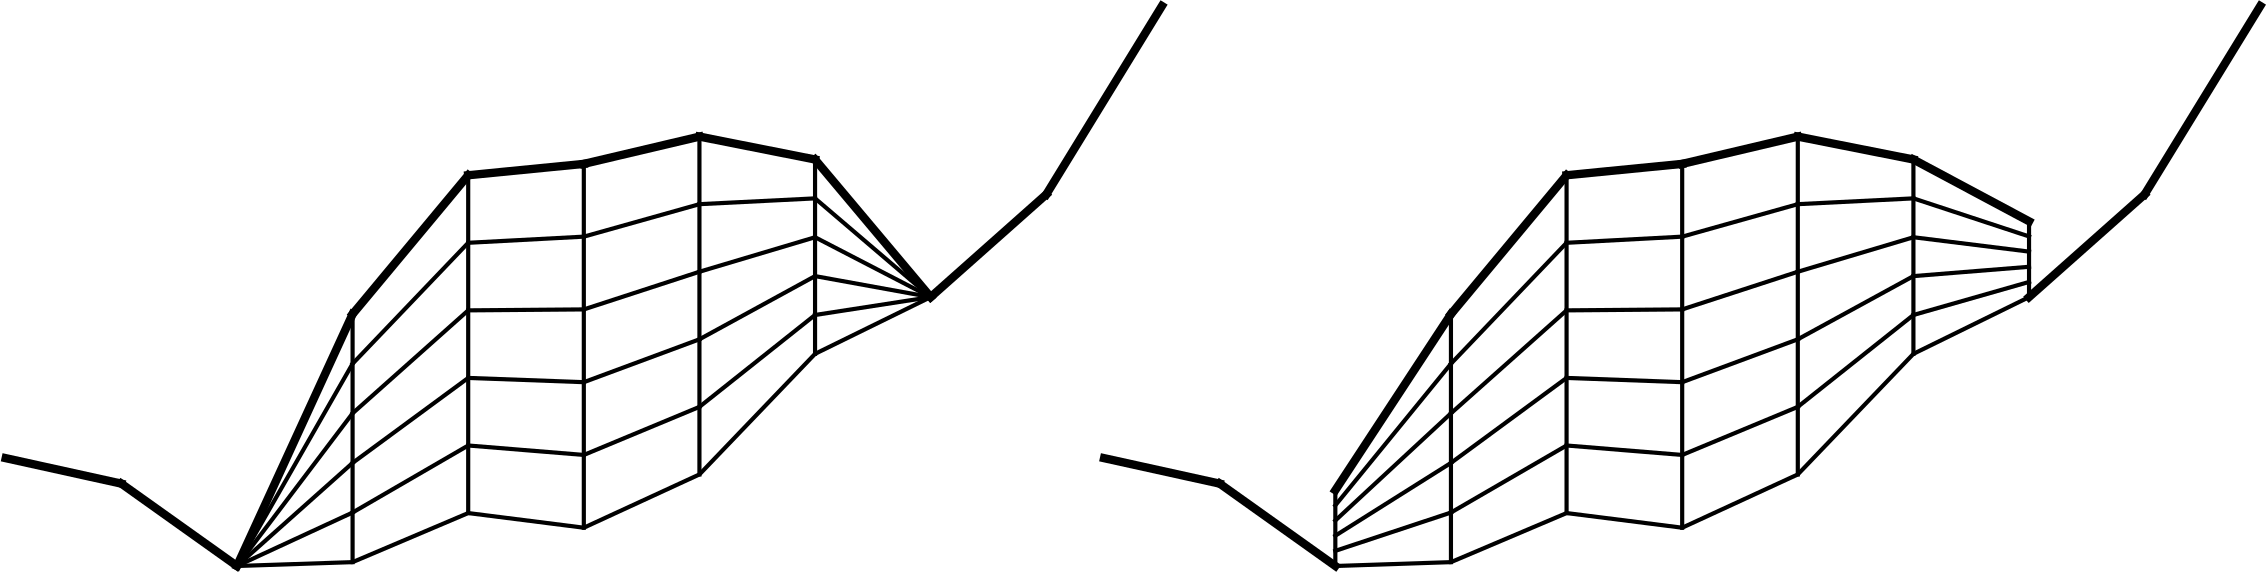
\includegraphics[width=\linewidth]{figs/extruded.png}
	\end{columns}
\end{frame}


\appendix

\begin{frame}{References}
	%\nocite{*} % Display all references regardless of if they were cited
	\bibliography{../paper/msg.bib}
	\bibliographystyle{plain}
\end{frame}


\end{document}
